\section*{Introduction}
		\paragraph{}
		Dans ce chapitre, nous présentons les résultats des simulations faites pour tester
		le fonctionnement de notre solution. Dans un premier temps, nous allons présenter quelques fonctionnalités développées dans l’application et nous aborderons ensuite une discussion.
		
		
		\section{Présentation des résultats des tests}
			\paragraph{}
				Pour réaliser les simulations, nous avons choisi d'utiliser deux machines toutes linux; l'une sous kali linux 2.0 Rolling, l'autre sous ubuntu 16.04 LTS. 
				\paragraph{}
				\begin{figure}[H]
					\begin{center}
					    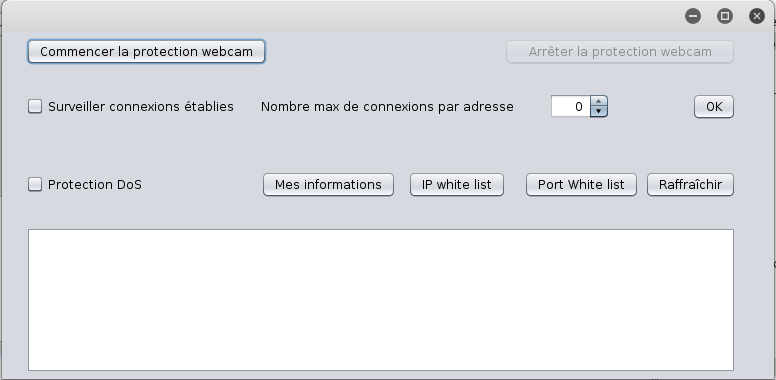
\includegraphics[scale=0.5]{images/accueil.png}
					\end{center}
					\caption{Ecran d'accueil de notre solution}
					\label{Accueil}
				    \end{figure}
				    Cette figure présente l'écran à l'ouverture de notre logiciel avec les différentes options. Lorsque l'utilisateur clique sur whitelist IP, il est redirigé vers une autre page dont l'image suit.
				     \begin{figure}[H]
					\begin{center}
					    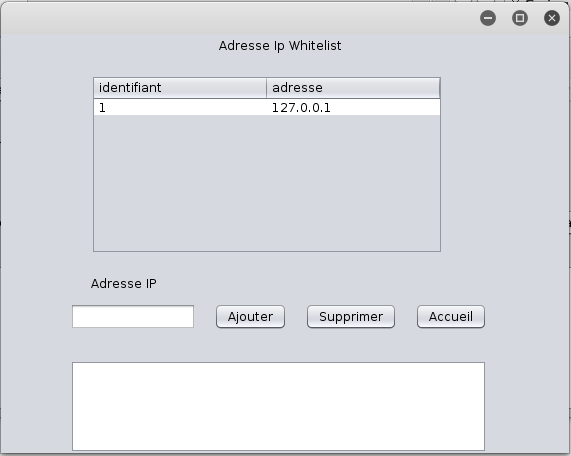
\includegraphics[scale=0.5]{images/ipwhitelist.png}
					\end{center}
					\caption{Page de la whitelist IP}
					\label{Page de la whitelist IP}
				    \end{figure}
				    Lorsqu'il clique sur le bouton réservé à la whitelist des ports, il est renvoyé vers un autre écran dont l'image suit.
				    \begin{figure}[H]
						\begin{center}
					    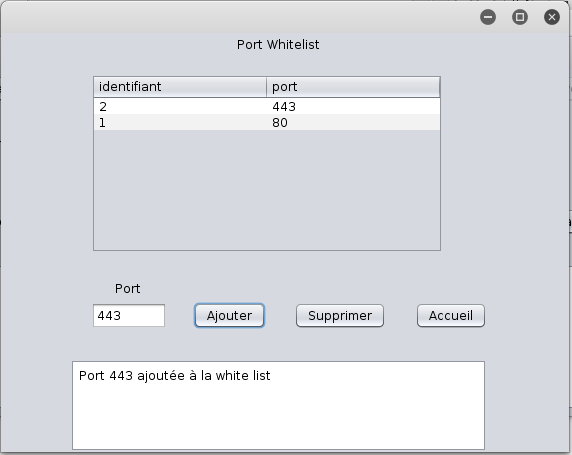
\includegraphics[scale=0.5]{images/portwhitelist.png}
					\end{center}
					\caption{Page de la whitelist Port}
					\label{Page de la whitelist Port}
				    \end{figure}
		Les données visualisées sont présentes parce qu'elles ont été entrées préalablement dans la base de données.
		\section{Cas pratique}
		Notre machine cible reçoit un mail comportant un lien pour voir les nouveautés de la communuauté Ubuntu. Après un clic sur le lien, il est redirigé vers un site ressemblant fortement à \url{community.ubuntu.com}, celui de la communauté Ubuntu, mais qui n'est rien d'autre qu'un site piégé dont voici l'aperçu.
		 \begin{figure}[H]
					\begin{center}
					    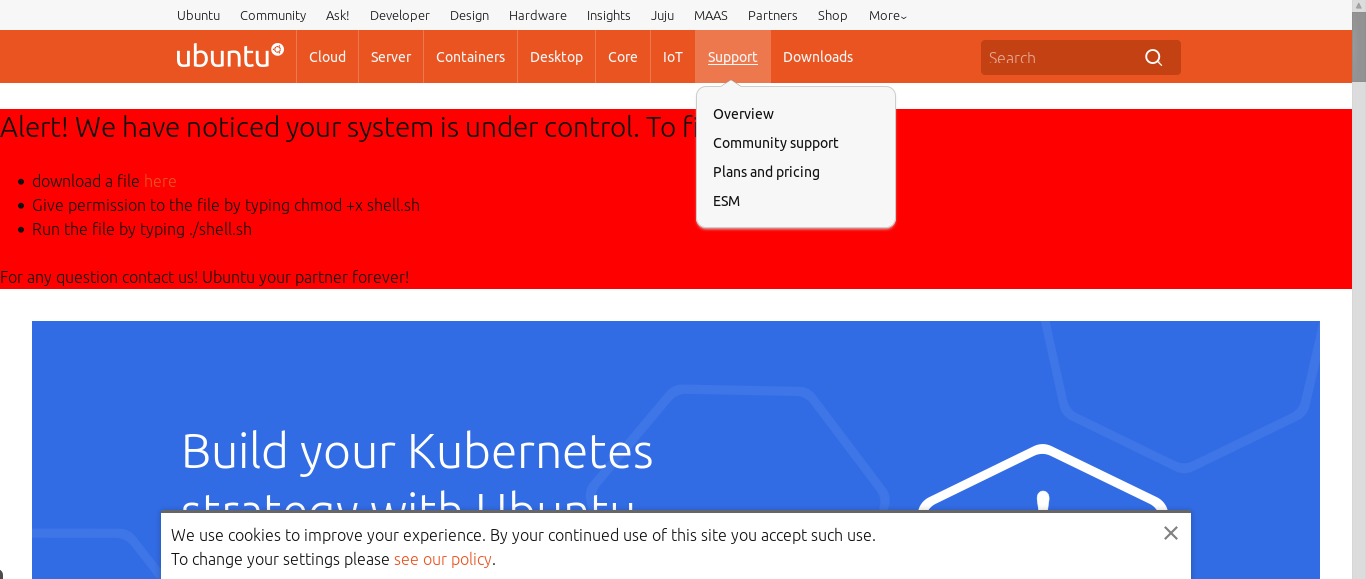
\includegraphics[scale=0.5]{images/fakeubuntu.png}
					\end{center}
					\caption{Faux site conçu par l'attaquant}
					\label{Site web piegé}
				    \end{figure}
		L'attaquant ajoute du contenu qui fait croire à la victime que son poste est sous contrôle et qu'il faudrait télécharger et exécuter un fichier contenant un script. Cela met la victime en confiance puisque, selon lui, il est audité depuis la communauté Ubuntu. Cependant, il ne fait que se piéger. L'attaquant utilise le framework Metasploit \cite{E} pour lancer une écoute de session (listener\footnote{Un listener est un composant de Metasploit qui attend une connexion entrante de tout type.}) vers toute cible essayant d'exécuter le fichier supposé résoudre le problème  notifié sur le faux site. Après exécution du fichier, l'attaquant prend possesion  de la machine cible.
		
		\begin{figure}[H]
					\begin{center}
					    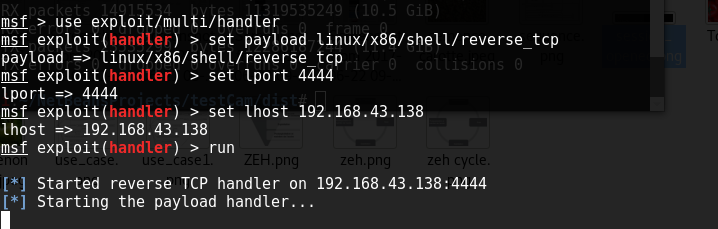
\includegraphics[scale=0.5]{images/session_listened.png}
					\end{center}
					\caption{Session en attente.}
					\label{Session en attente}
				    \end{figure}
		  \begin{figure}[H]
					\begin{center}
					    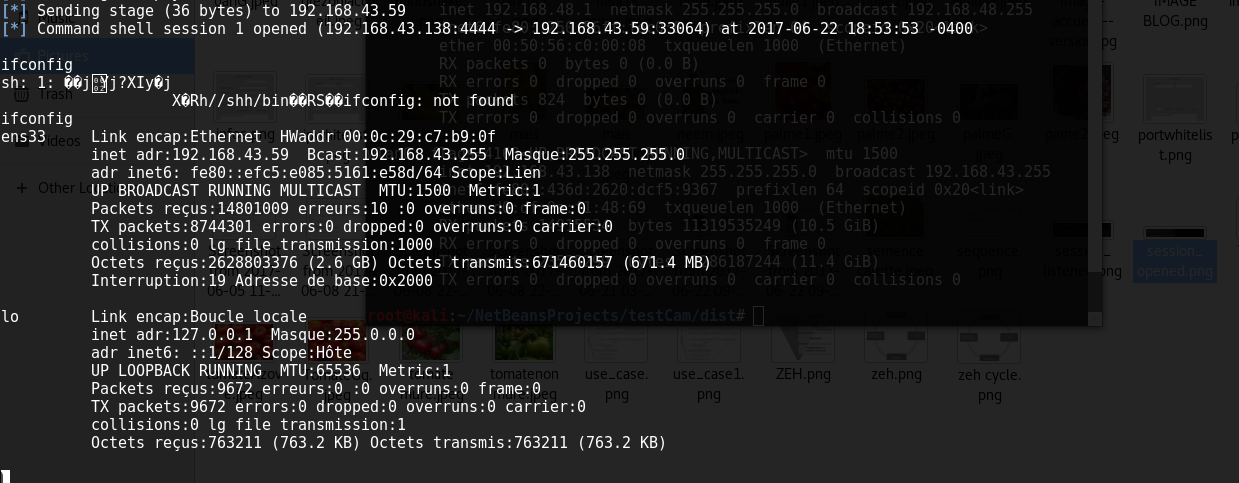
\includegraphics[scale=0.5]{images/session_opened.png}
					\end{center}
					\caption{Session ouverte vers la machine cible.}
					\label{Session ouverte}
				    \end{figure}
				    
Lorsque l'utilisateur de la machine cible active la détection d'intrusions, une alerte lui est envoyée en précisant la connexion établie.
 \begin{figure}[H]
					\begin{center}
					    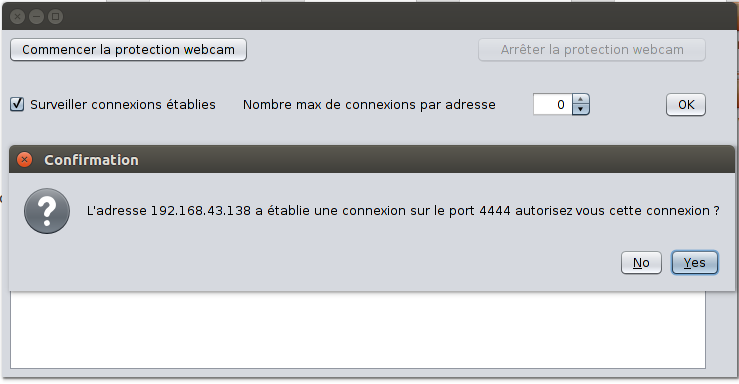
\includegraphics[scale=0.5]{images/session_detected.png}
					\end{center}
					\caption{Alerte connexion établie}
					\label{Connexion établie }
				    \end{figure}
				    
				
		Ne reconnaissant pas cette connexion comme légale, l'utilisateur décide d'arrêter. Cela met fin à la connexion établie et met en liste noire l'adresse source de l'attaquant.
	
	\begin{figure}[H]
					\begin{center}
					    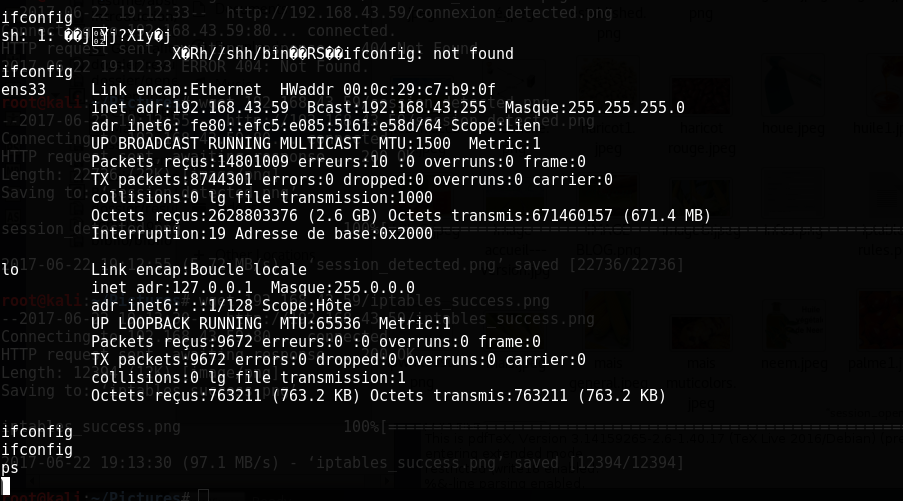
\includegraphics[scale=0.5]{images/session_notworking.png}
					\end{center}
					\caption{Les commandes du shell ne fontionnant plus}	
					\label{Les commandes du shell ne fontionnant plus}
				    \end{figure}
				    
				    
				    \begin{figure}[H]
					\begin{center}
					    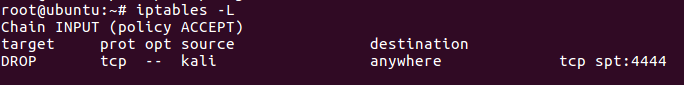
\includegraphics[scale=0.5]{images/iptables_success.png}
					\end{center}
					\caption{Adresse et port en blacklist}	
					\label{Blacklist}
				    \end{figure}
	\section{Discussion}
			\paragraph{}
				Notre projet est né de plusieurs constats généraux de l'ordre de la sécurité informatique pour la protection de l'information et de la vie privée.
				
				 Les recherches effectuées nous ont permis de constater l'existence de certaines solutions. Cependant, ces solutions, loin de contrer tout type d'intrusion, ne peuvent pas être prises pour seuls moyens de sécurité.
			\paragraph{}
				Notre solution apporte un outil de défense contre certaines attaques en réseau informatique parmi lesquelles l'espionnage par webcam, les intrusions clandestines, les dénis de service. Aussi permet-elle de lever le mythe selon lequel on est en sécurité absolue sur les systèmes Linux (un exemple se présente dans le cas pratique).
			\paragraph{}
				Ainsi, d'une part, notre solution est simple à utiliser et est accessible à un grand public, celui regroupant les utilisateurs Linux.
				Elle permet aux utilisateurs d'être informés de quelques processus tournant à leur insu.  
			\paragraph{}
				D'autre part, notre solution est exclusivement destinée aux systèmes Linux, ce qui représente une limite car, aujourd'hui beaucoup d'ordinateurs tournent sous les sytèmes Windows et Mac, sans compter la multiplicité des versions Linux qui existent.  
\section*{Conclusion}
			\paragraph{}
				Dans ce chapitre, nous avons exposé les résultats des tests de notre application et réalisé quelques critiques concernant ses performances et ses insuffisances. Ces insuffisances peuvent être perçues comme des perspectives afin d'améliorer le travail fait pour une utilisation plus éfficiente.